\section{Arrival time prediction methods}
\label{sec:prediction_arrival_time}




\begin{knitrout}\small
\definecolor{shadecolor}{rgb}{0.969, 0.969, 0.969}\color{fgcolor}\begin{figure}

{\centering 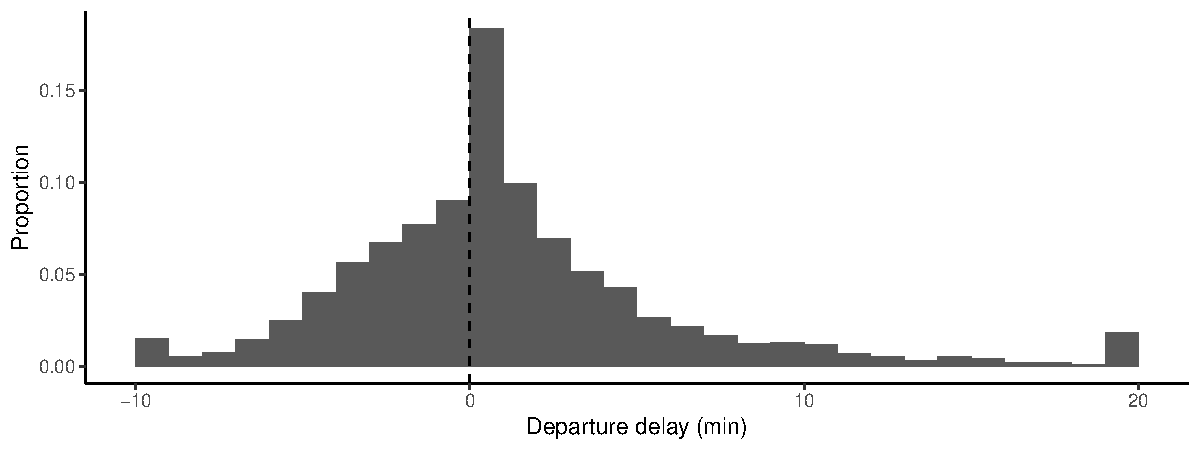
\includegraphics[width=\linewidth]{figure/layover_observance-1} 

}

\caption[Vehicle delays at layover stops]{Vehicle delays at layover stops truncated to 10~minutes early and 20~minutes late. Negative values indicate non-adherance by drivers, which make up 40\% of cases.}\label{fig:layover_observance}
\end{figure}


\end{knitrout}

The estimated trip state (and any associated vehicle) together with the road network can now be combined to forecast how long it will take for the vehicle to reach all remaining stops along the route. Dwell times can also affect arrival time uncertainty \citep{Shen_2013,Wang_2016,Robinson_2013,Meng_2013,Shalaby_2004,Hans_2015}. Some trips have the added complexity of layovers at specific stops---these are common at major points of interest, such as at a mall, or stations where many routes connect so passengers can transfer between services (see \cref{sec:gtfs}). In theory, drivers wait at these stops until the scheduled departure time before continuing the trip; however, in 40\% of cases over two weeks, the driver left before the scheduled departure time, as is demonstrated in \cref{fig:layover_observance}, and 31\% departed more than one minute early.


There are various ways to forecast arrival times, each with associated drawbacks and advantages. This section presents four arrival time prediction methods:
\begin{itemize}
\item \Fpf{} uses the particle filter estimate of vehicle state and the network state to obtain arrival time distributions;
\item \Fnorm{} uses a normal approximation of the vehicle's state, along with trip state, network state, and dwell-time distributions;
\item \Fhist{} uses only historical delay data; and
\item \Fsched{} uses the schedule and current real-time delay, which is currently used by \AT{}.
\end{itemize}


Methods \Fpf{} and \Fnorm{} use the network state, which is simplified for each route by including only the segments (in order) used by route $r$ with mean and variance
\begin{equation}
\label{eq:route_nw_state}
\RouteNWstate^r =
\begin{bmatrix}
\RouteNWstateseg^r_1 \\
\RouteNWstateseg^r_2 \\
\vdots \\
\RouteNWstateseg^r_L
\end{bmatrix}\quad\text{and}\quad
\RouteNWstatevar^r =
\begin{bmatrix}
\RouteNWstatevarseg^r_{1} & \RouteNWstatecor^r_{1,2} & \cdots &\RouteNWstatecor^r_{1,L} \\
\RouteNWstatecor^r_{2,1} & \RouteNWstatevarseg^r_{2} & \ddots &\RouteNWstatecor^r_{2,L} \\
\vdots & \ddots & \ddots & \vdots \\
\RouteNWstatecor^r_{L,1} & \RouteNWstatecor^r_{L,2} & \cdots & \RouteNWstatevarseg^r_L
\end{bmatrix},
\end{equation}
respectively, where $\RouteNWstateseg^r_{i}$ is the average vehicle speed along the $i$th segment of route $r$, $\RouteNWstatevarseg^r_{i}$ is the variance for that segment, and $\RouteNWstatecor^r_{i,j}$ is the covariance between segments $i$ and $j$. Note that the current implementation does not include segment covariances, but the above set-up demonstrates that the model can include them, if available. To simplify notation, I have dropped the $r$ superscript for the remainder of this chapter since only one route is considered at any one time.

For bus stop dwell times, we collected two weeks of data (as in \cref{sec:nw_par_est}) and calculated the mean and variance of dwell time for all stops along each trip. It is possible to determine if a bus \emph{did} stop (there is both an arrival and a departure time), but not that a bus \emph{did not} stop. For example, if the bus reports only an arrival time, it is unclear whether this is because the bus truly did not stop, or if it is a deficiency with the data. The bus may not have reported both observations, or, more likely, the polling interval (30 seconds) did not see both of them (Auckland Transport's real-time feed only includes the most recent observation). Therefore, stopping probabilities cannot be estimated from the data, so the same value of $\Prstop_j=0.5$ is used as in \cref{cha:vehicle_model}.


\subsection{Particle filter (\Fpf{})}
\label{sec:prediction_arrival_time_pf}

Each active trip is associated with a single vehicle, itself associated with a set of  $\Np$~particles approximating the vehicle's state. Perhaps the most straightforward method---at least conceptually---of predicting arrival times is to let each particle progress to the end of the route and record its arrival times. Computationally, this is easy to implement but very intensive, significantly increasing iteration time for the application. However, as we no longer need to worry about updating (via importance resampling), we can use a smaller subset of particles, $\Np^\star \leq \Np$, which can be adjusted depending on how many stops there are along the remainder of the route.

\begin{itemize}
\item better argument for using smaller $N$
\item rewrite paragraph below more succinctly (perhaps as a list)
\item for the dwell time stuff, refer back to Ch 3
\end{itemize}


To implement the particle filter forecast method, which we denote \Fpf{}, we take a (weighted) subsample of $\Np^\star$ particles at time $\Vtime_k$, $\tilde\Vstate_k$ (the time of the most recent vehicle observation). For each particle, we calculate the arrival time at each upcoming stop. First, if the particle is at a stop,  the ``remaining travel time'' for the current segment is needed, which we calculate by taking the particle's current speed, adding some noise, and extrapolating to the end of the segment. Having completed the current (partial) segment $j$, the particle's travel time to stop $j$, $\Linkt\vi_j$, is used to estimate the arrival time,
\begin{equation}
\label{eq:particle_arrival_time}
\Tarr\vi_j = \Vtime + \Linkt\vi_j.
\end{equation}
Next, we iteratively add dwell time and travel time for stops and road segments, respectively, until the particle reaches the end of the route; alternatively, we could stop after some number of stops, as we discuss in \cref{sec:prediction_performance}. The dwell time is assumed Gaussian with mean and variance estimated from historical data, $\mu_{\dwell_j}$ and $\sigma_{\dwell_j}$, respectively:
\begin{equation}
\label{eq:prediction_dwell_time}
\begin{split}
\Istop\vi_j &\sim \Bern{\Prstop_j} \\
\pserve\vi_j &\sim \TNormal{\mu_{\dwell_j}}{\sigma_{\dwell_j}}{0}{\infty} \\
\pdwell\vi_j &= \Istop\vi_j \pserve\vi_j
\end{split}
\end{equation}


\begin{itemize}
\item better clarification of terms here
\end{itemize}

When estimating travel time, the particle's speed along each segment is drawn from the network state,
\begin{equation}
\label{sec:particle_travel_time_pred}
\Linkt\vi_j \sim
\Normal{\hat\RouteNWstateseg_j}{
  (P_j + \Delta_j\NWnoise)^2)\wedge\mu_{P_j}
},
\end{equation}
which allows uncertainty to increase for more temporally distant forecasts, with a maximum set by the historical (prior) uncertainty.


Having obtained arrival times for all $\Np^\star$ particles, the predictive distribution for stop $j$---as in \cref{cha:vehicle_model}---is simply
\begin{equation}
\label{eq:particle_predictive_dist}
p(\Tarr_j | \Tripr_k, \RouteNWstate_\Tripr) \approx
\sum_{i=1}^{\Np^\star} \Pwt \dirac_{\Tarr_j\vi}\left(\Tarr_j\right)
= \frac{1}{\Np^\star}\sum_{i=1}^{\Np^\star} \dirac_{\Tarr_j\vi}\left(\Tarr_j\right)
\end{equation}
since all weights are equal. From the particle approximation of the distribution of arrival times we obtain point estimates or quantiles---for example, the mean, median, or a 90\% credible region. As discussed in \cref{app:particle-summaries}, computing quantiles (including the median) is a computationally demanding task for large numbers of particles due to the necessity to sort the particles in order from earliest to latest arrival times---at each stop.

\subsection[Normal approximation]{Normal approximation (\Fnorm{})}
\label{sec:prediction_arrival_time_normal}

Due to the computational demand of the particle filter, significant speed improvements can be obtained by using a normal approximation instead. The network state is a multivariate normal random variable, so the issue lies with stop dwell times having a point mass at zero, resulting in a mixture predictive distribution. For each stop the vehicle passes, there are twice as many components, so after $m$ stops, there are $2^m$ components. However, these regularly converge after a few stops, as shown in \cref{fig:normal_approx}.

\begin{knitrout}\small
\definecolor{shadecolor}{rgb}{0.969, 0.969, 0.969}\color{fgcolor}\begin{figure}

{\centering 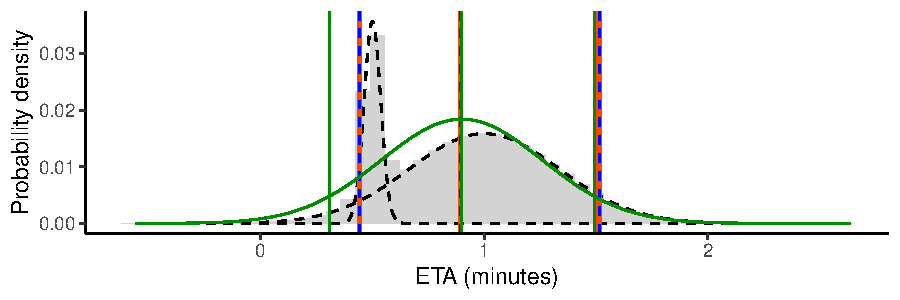
\includegraphics[width=\textwidth]{figure/normal_approx-1} 

}

\caption[Normal approximation for a series of stops ahead]{Normal approximation for a series of stops ahead. The true distribution is shown by the histogram with the underlying components (dashed curves). The vertical lines represent the quantiles computed using the sampled data, the normal mixture (using the optimisation formula), or a single normal approximation.}\label{fig:normal_approx}
\end{figure}


\end{knitrout}

A mixture of normal distributions can approximate the arrival time distribition \citep{Wang_2012} by expressing the mean and uncertainty as vectors $\tilde\mu$ and $\tilde\sigma^2$, respectively, along with a third vector $\tilde\pi$ denoting the $\tilde N$ mixture weights\footnote{We are using the tilde over parameters, e.g., $\tilde x$, to help distinguish them from others used throughout the thesis}, such that
\begin{equation}
\label{eq:ch5:mixture_weight_spec}
\tilde\pi_i > 0, i = 1, \ldots, \tilde N
\text{ and } \sum_{i=1}^{\tilde N} \tilde\pi_i = 1.
\end{equation}
The arrival time at stop $j + n$ is then given by
\begin{equation}
\label{eq:arrival_time_normal_approx}
\Tarr_{j+n} | \tilde\mu, \tilde\sigma^2, \tilde\pi, \RouteNWstate =
\sum_{\ell=j}^{j+n-1} \RouteNWstateseg_\ell +
\sum_{i=1}^{\tilde N} \tilde\pi_i z_i,\quad
z_i \sim \Normal{\tilde\mu_i}{\tilde\sigma^2_i}.
\end{equation}


Each component $i$ has an indicator $I_{im} = \{0,1\}$ of whether or not it stopped at stop $m$, so the total dwell time has mean and variance
\begin{equation}
\label{eq:mixture_dwell_times}
\tilde\mu_i = \sum_{m=j}^{j+n} I_{im} \dwell_m\quad\text{and}\quad
\tilde\sigma_i^2 = \sum_{m=j}^{j+n} I_{im} \dwellvar_m,
\end{equation}
respectively, assuming dwell times at individual stops are independent of each other.

Mixture weights are obtained through the stopping probability at each stop, $\pi_j$:
\begin{equation}
\label{eq:ch5:mixture_weights}
\tilde\pi_i = \prod_{m=j}^{j+n} \tilde p_{im}
\end{equation}
where
\begin{equation}
\label{eq:ch5:mixture_weights2}
\tilde p_{im} =
\begin{cases}
\pi_m & \text{if } I_{im} = 1 \\
1 - \pi_m & \text{otherwise.}
\end{cases}
\end{equation}


The mixture approximation works well for a few stops ahead, but after some time the mixture weights become small and the components combine, as shown in \cref{fig:normal_approx}. To prevent $\tilde N$ from becoming too large, the full distribution is simplified into a single component with mean and variance
\begin{equation}
\label{eq:mixture_mean}
\begin{split}
\E{\Tarr_m | \tilde\pi, \tilde\mu, \tilde\sigma^2, \RouteNWstate} &=
\E{\sum_{\ell=j}^{j+n-1} \RouteNWstateseg_\ell +
  \sum_{i=1}^{\tilde N} \tilde\pi_i z_i} \\
&= \sum_{\ell=j}^{j+n-1} \E{\RouteNWstateseg_\ell} +
  \sum_{i=1}^{\tilde N} \tilde\pi_i \E{z_i} \\
&= \sum_{\ell=j}^{j+n-1} \hat\RouteNWstateseg_\ell +
  \sum_{i=1}^{\tilde N} \tilde\pi_i \tilde\mu_i
\end{split}
\end{equation}
and
\begin{equation}
\label{eq:mixture_variance}
\begin{split}
\Var{\Tarr_m | \tilde\pi, \tilde\mu, \tilde\sigma^2, \RouteNWstate} &=
\Var{\sum_{\ell=j}^{j+n-1} \RouteNWstateseg_\ell +
  \sum_{i=1}^{\tilde N} \tilde\pi_i z_i} \\
&= \sum_{\ell=j}^{j+n-1} \Var{\RouteNWstateseg_\ell} +
  \sum_{i=1}^{\tilde N} \tilde\pi_i^2 \Var{z_i} \\
&= \sum_{\ell=j}^{j+n-1} \hat\RouteNWstatevarseg_\ell +
  \sum_{i=1}^{\tilde N} \tilde\pi_i \tilde\sigma_i^2
\end{split}
\end{equation}
respectively, assuming segment travel time and dwell time are independent---assuming otherwise makes this model impossible to work with; indeed, this model versus the particle filter (which makes no such assumption) is effectively testing the viability of this assumption.


An optimisation is used to obtain quantiles $q_\alpha$ such that
\begin{equation}
\label{eq:mixture_quadratic}
\left[
  p\left(\alpha \leq \Tarr_m | \tilde\pi, \tilde\mu, \tilde\sigma^2, \RouteNWstate\right) - q_\alpha
\right]^2 = 0.
\end{equation}
This is straightforward using Brent's Algorithm \citep{Brent_1971}, implemented in the Boost \textsf{C++} library.

When the 2.5\%, 50\%, and 97.5\% quantiles for the single approximation are within 30~seconds of the same quantiles computed for the mixture distribution, the mixture is replaced with one single component with mean and variance defined in \cref{eq:mixture_mean,eq:mixture_variance}. In some situations, the mixture may not converge into a single distribution quick enough, so to prevent the number of components $\tilde N$ from exceeding $2^8=256$, all components with weights less than a predefined threshold (we used $\frac{1}{2}\max_i(\pi_i)$) are combined into a single component.


%%%%%%%%%%%%%%%%%%%%%%%%%%%%%%%%%%%%%%%%%%%%%%%%%%%%%%%%% Historical data
\subsection[Historical arrival delays]{Historical arrival delays (\Fhist{})}
\label{eq:prediction_arrival_historical}

Another way to make predictions is to use historical data instead of real-time. We collected two weeks of data and recorded arrival time delays by stop and route to obtain a distribution which can then be used to make predictions. The arrival time at stop $j$ along route $r$ has an average delay of $\bar d_{rj}$ seconds with variance $D_{rj}^2$, so the predicted arrival time at stop $j$ on route $r$ with scheduled arrival time $S_{rj}$ is
\begin{equation}
\label{eq:arrival_pred_historical}
\hat\Tarr_{j} \sim \Normal{S_{rj} + \bar d_{rj}}{D_{rj}^2}.
\end{equation}


%%%%%%%%%%%%%%%%%%%%%%%%%%%%%%%%%%%%%%%%%%%%%%%%%%%%%%%%% Schedule + delay
\subsection[Schedule delays]{Schedule delays (\Fsched{})}
\label{eq:prediction_arrival_sched_delay}

The currently deployed prediction method uses the scheduled arrival time at stop $j$ along route $r$, $S_{rj}$, along with the arrival or departure time at the most recently visited stop, $T_{rm}$, giving a current delay, in seconds, of
\begin{equation}
\label{eq:sched_cur_delay}
d_{r} = T_{rm} - S_{rm}.
\end{equation}
The arrival time is then predicted as
\begin{equation}
\label{eq:sched_pred_arr}
\hat\Tarr_{rj} = S_{rj} + d_r.
\end{equation}
Note, however, that if a trip has not yet been observed, the default delay is $d_r = 0$. This happens if there is not a vehicle servicing it, the vehicle is running late, or the trip has been cancelled altogether.
